\documentclass[compress]{beamer}
\usepackage{beamerthemeproyxetex}


\title{CLAM: Computational Linguistics Application Mediator}
\author{Maarten van Gompel}
\date{20 Mei 2010}
\usepackage{graphicx}


\begin{document}

\begin{frame}
	\titlepage\smallraccoon\ilkuvt
\end{frame}

\section{Introduction}

\subsection{Introduction}
\begin{frame}{Introduction}

    \begin{block}{Observation}
        There are a lot of specialised command-line NLP tools available.
    \end{block}

    \begin{block}{Problems}
        \begin{enumerate}
            \item Tools often available only locally, installation and configuration can be tough
            \item Not very user-friendly for the untrained general public or technically-challenged researchers (aka Linguists)
            \item How to connect one tool to another?
        \end{enumerate}
    \end{block}
\end{frame}


\subsection{Solution}
\begin{frame}
    \begin{block}{Solution} 
        Making NLP tools available as a full-fledged webservice.
    \end{block}

    \begin{block}{Advantages}

        \begin{enumerate}
            \item Services available over the web.
            \item User-friendly interface built-in in the webservice
            \item Great for demo purposes
            \item Multiple webservices can be chained in a workflow
        \end{enumerate}

    \end{block}
\end{frame}


\subsection{Our Focus}
\begin{frame}
    \begin{block}{Our Focus}
   
        \begin{enumerate}
            \item A \emph{universal} approach: \emph{wrapping}
            \begin{itemize}
                \item Turn almost \emph{any} NLP tool into a webservice with \emph{minimal effort}
                \item NLP tool = Given input files and a custom set of parameters, produce output files
                \item No need to alter the tool itself
            \end{itemize}
            \item Machine-parsable interface \& Human-friendly interface
        \end{enumerate}
    
    \end{block}
\end{frame}


\subsection{Wrapping Approach}
\begin{frame}

    \begin{block}{Wrapping Approach}

        %TODO: insert fancy picture of an open clam
       
        \begin{enumerate}
            \item NLP application: blackbox
            \item Wrapper script
            \item CLAM Webservice
            %\item CLAM Interface
        \end{enumerate}

    \end{block}


\end{frame}


\section{Technical Details}

\begin{frame}{Technical Details}


    \begin{block}{RESTful Webservice}
        
        RESTful Webservice (as opposed to SOAP, XML-RPC)

        \begin{enumerate}
            \item Resource-oriented: "Representations" of "resources" (projects)
            \item Using HTTP verbs
            \item Lightweight
            \item Returns human-readable, machine-parseable XML adhering to a CLAM XML Scheme Definition %TODO: XSD not written yet
            \item User authentication in the form of HTTP Digest Authentication
        \end{enumerate}    
    \end{block}
\end{frame}

\begin{frame}
    \begin{block}{Python}
            Written entirely in Python 2.5

            \begin{enumerate}
                \item NLP tools, wrapper scripts, and clients may be in any language 
                \item But: Readily available API when writing wrapper scripts and clients in Python.
                \item Built on web.py, runs standalone and out-of-the box with built-in CherryPy webserver        
            \end{enumerate}

    \end{block}
\end{frame}


\begin{frame}
    \begin{block}{Built-in User Interface}

            User interface automatically generated from XML using XSLT (in browser)

            \begin{enumerate}
                \item Webservice \emph{directly} accessible from webserver
                \item Web 2.0 interface: xHTML Strict, jquery (javascript), AJAX, CSS
            \end{enumerate}

            %Insert user-interface screenshot?

    \end{block}
\end{frame}



\section{Setup}

\subsection{Setup}

\begin{frame}{Setup}
    \begin{block}{CLAM Setup}

            Projects are the main resources, users start a new project for each experiment/batch.
    
            \textbf{Three states}:

            \begin{itemize}
                \item \textbf{Status 0)} Parameter selection and file upload
                \item \textbf{Status 1)} System in progress
                \begin{itemize}
                    \item Actual NLP tool runs at this stage only
                    \item Users may safely close browser, shut down computer, and come back later in this stage
                \end{itemize}
                \item \textbf{Status 2)} System done, view/download output files
            \end{itemize}

            %Insert user-interface screenshot?

    \end{block}
\end{frame}

\subsection{Providing a Service}

\begin{frame}
    \begin{block}{Providing a Service}
        In order to make a webservice:
        \begin{enumerate}
            \item Write a service configuration file \footnotesize{(in Python, but no Python experience required)}. 
            \begin{itemize}
                \item General meta information about your system \footnotesize{(name, description, etc..)}
                \item Definition of parameters accepted by your system/wrapper script
                \item Definition of input formats and output formats
                \item Definition of users and authentication method
            \end{itemize}
            \item Write a wrapper script for your system
            \begin{itemize}
                \item Wrapper script is invoked by CLAM, and should in turn invoke the actual system
                \item Acts as glue between CLAM and your NLP Application.
                \item Can be written in any language (python users may benefit from the CLAM API)
                \item Not always necessary, NLP applications can be invoked directly by CLAM as well.
            \end{itemize}
        \end{enumerate}
    \end{block}

\end{frame}


\subsection{Writing a Client}

\begin{frame}
    \begin{block}{Writing a Client}
        \begin{enumerate}
            \item Communicate with service over HTTP, using HTTP verbs on projects and files to effectuate state transfers 
            \begin{itemize}
                \item \texttt{GET /} - List all projects
                \item \texttt{GET /project/} - Get a project's state
                \item \texttt{PUT /project/} - Create a project
                \item \texttt{POST /project/} - Start a project with POSTed data as parameters
                \item \texttt{DELETE /project/} - Delete or abort a project
                \item \texttt{POST /project/upload/} - Upload a file
                \item \texttt{GET /project/output/} - Download all output files as archive
                \item \texttt{GET /project/output/file} - Download output file
            \end{itemize}
            \item Parse XML responses
            \item \textbf{Python users benefit from CLAM Client API, taking care of all above communication and response parsing!}
        \end{enumerate}
    \end{block}

\end{frame}


\subsection{Architecture}

\begin{frame}
    \begin{block}{Architecture}
        \begin{figure}[h]
        \begin{center}
        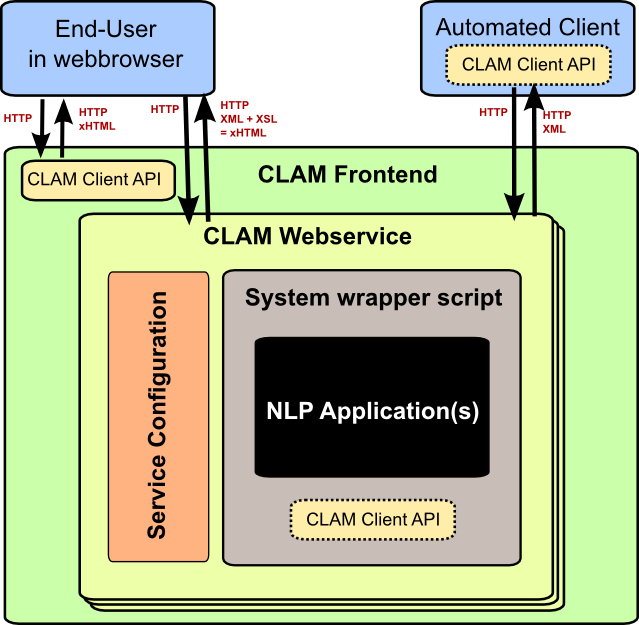
\includegraphics[width=70.0mm]{architecture.png}
        \end{center}
        \caption{The CLAM Architecture}
        \label{fig:arch} 
        \end{figure}

    \end{block}
\end{frame}

\section{End}


\begin{frame}
    \raccoon
\end{frame}



\end{document}
